% 续写《单层 TMD 材料的三能带紧束缚模型构建》：
% 三能带模型的 GW 参数拟合、Keldysh 屏蔽势与 Bethe-Salpeter 方程
% 编译：xelatex theory.tex（中文由 ctex 处理，需要 TeX Live 的 ctex 包）
\documentclass[11pt,a4paper]{ctexart}

\usepackage{amsmath,amssymb,bm}
\usepackage{booktabs}
\usepackage{graphicx}
\usepackage{float}
\usepackage{geometry}
\usepackage{xcolor}
\usepackage[colorlinks=true,linkcolor=blue!45!black,citecolor=blue!45!black,urlcolor=blue!45!black]{hyperref}
\geometry{margin=2.6cm}
\graphicspath{{fig/}}

% 章节状态标记：全部做完后把这两个宏改成空 \newcommand{\done}{} 即可一次去掉
\newcommand{\done}{（已完成）}
\newcommand{\todo}{（待完成）}

\newcommand{\kk}{\mathbf{k}}
\newcommand{\kq}{\mathbf{k}'}
\newcommand{\qq}{\mathbf{q}}
\newcommand{\RR}{\mathbf{R}}
\newcommand{\eps}{\varepsilon}
\newcommand{\dd}{\mathrm{d}}
\newcommand{\ii}{\mathrm{i}}

\title{单层 TMD 三能带紧束缚模型的续篇\\[2mm]
\large 从 GW 能带重新拟合参数到 GW-BSE 激子}
\author{}
\date{\today}

\begin{document}
\maketitle

\begin{abstract}
上一篇\footnote{《单层 TMD 材料的三能带紧束缚模型构建》，\url{https://ionizing.page/post/tmd-tightbinding/}。}
从对称性出发建立了单层 TMD 的三能带紧束缚模型，
并讨论了它的适用范围。
这一篇接着往下走。把 19 个参数拟合到 GW 准粒子能带，
在拟合好的模型上引入 Keldysh 型二维屏蔽库仑势，
求解 Bethe-Salpeter 方程得到激子能级，最后与 VASP 的 BSE 结果对照。
文中给出每一步的公式、本课题采用的数值，以及公式与程序模块的对应关系。
\end{abstract}

\tableofcontents
\newpage

%=====================================================================
\section{引子}

\subsection{上一篇停在哪里}

上一篇完成了三能带模型的完整构建。
它先分析单层 TMD 的 $D_{3h}$ 对称性，
据此确定 Mo 原子的 $d_{z^2}$，$d_{xy}$，$d_{x^2-y^2}$ 三个轨道构成基组，
然后由对称性操作把跳跃矩阵的独立参数压缩到 19 个，
即原位能两个，最近邻六个，次近邻五个，第三近邻六个。
模型建成之后，参数直接取自文献~\cite{liu2013}，用它们复现了能带结构。
最后一节讨论了模型的适用范围，
指出三能带近似在 $\Gamma$ 谷附近以及远离 $K/K'$ 的区域会失效。

文献参数对应的是 DFT 层面的单粒子能带。
做激子计算需要准粒子能带，所以本学期的第一步是把这 19 个参数
重新拟合到 GW 能带，给后面的 BSE 一个正确的单粒子起点。

\subsection{三个目标与章节对应}

课题开始时定下的三个目标是下面这样。为了不用每次回去翻论文，这里把每条目标
涉及的主要式子也一并写出来，完整的推导与实现放在后面的对应章节。

\begin{enumerate}
  \item \textbf{实现 GW 能级的三带紧束缚模型。}
        模型结构完全不动，只把参数重新拟合到 GW 能带，也就是解
        \[
        \min_{\mathbf p}\ \sum_{n,\kk}\big[E_{\mathrm{TB}}(n,\kk;\mathbf p)
        -E_{\mathrm{GW}}(n,\kk)\big]^2 ,
        \]
        其中 $\mathbf p$ 是 19 个参数，即两个原位能、六个 $t$、五个 $r$、六个 $u$。
        GW 能带与模型本征值都是按能量排序输出的，
        所以这一步还包含把排序能级接回物理能带，并确定模型的哪条带对哪条物理带。

  \item \textbf{实现论文式~(6) 的 BSE 核}，即
        \[
        W^{(d)}_{cv\kk,c'v'\kq}
        =u(\kk-\kq)\,I^{*}_{c'\kq,c\kk}\,I_{v'\kq,v\kk} .
        \]
        核里是两个因子相乘。屏蔽库仑势 $u(q)$ 取 Keldysh 形式，
        需要先定下 $r_0$ 与 $\eps_d$ 两个介电环境参数（第~\ref{sec:keldysh}~节）；
        轨道交叠 $I_{a\kq,b\kk}=\sum_\alpha C^{a*}_{\alpha\kq}C^{b}_{\alpha\kk}$
        由本征矢给出（式~\eqref{eq:overlap}），因为 $I$ 不是规范不变量，
        用之前要先固定本征矢的相位。
        实现时还要处理 $\kk=\kq$ 处 $u(0)$ 的发散（式~\eqref{eq:reg}），
        那是 $\kk=\kq$ 那个对角元的数值处理，不属于式~(6) 本身。

  \item \textbf{解论文式~(5) 的 BSE}，得到激子能级，
        \[
        E_{cv\kk}A^{M}_{cv\kk}
        +\frac{1}{V}\sum_{c'v'\kq}W_{cv\kk,c'v'\kq}A^{M}_{c'v'\kq}
        =E_{M}A^{M}_{cv\kk},
        \qquad V=A_cN_k^2 ,
        \]
        也就是把一个 $N_k^2N_cN_v$ 维的复厄米矩阵对角化，
        再把最低的若干条 $E_M$ 与 VASP 的 BSE 本征值（\texttt{BSEEIGS.dat}）对照。
\end{enumerate}

三条目标、章节与完成状态的对应关系列在表~\ref{tab:goals}。

\begin{table}[htbp]
\centering
\caption{三个目标与章节的对应。状态栏与各节标题上的标记一致。}
\label{tab:goals}
\begin{tabular}{@{}clll@{}}
\toprule
目标 & 主要工作 & 章节 & 状态\\
\midrule
1 & 重拟合 19 个参数；能带身份与导带配对 &
    \S4、\S5 & 已完成\\
2 & 实现式 (6)：$u(q)$ 与 $I$ 两个因子 &
    \S6、\S7.1--\S7.3 & 待完成\\
3 & 对角化得激子能级，与 \texttt{BSEEIGS.dat} 对照 &
    \S7.4、\S10 & 待完成\\
\bottomrule
\end{tabular}
\end{table}

论文式~(11)--(16) 的光学响应不在三个目标之内，属于做完激子能级之后的下一步，
放在 \S8。

工作流程是先在单粒子层面把模型修好，再在同一个模型上叠加电子-空穴相互作用。
这样做的好处是单粒子部分的误差与相互作用部分的误差可以分开检验，
出了问题能定位到具体环节。

%=====================================================================
\section{记号与约定}

本篇沿用上一篇的记号，只把用到的部分列在下面，其余的推导见上一篇。

晶格常数记作 $l$，取 $\mathrm{MoS_2}$ 的实验值 $l=3.182164$~\AA{}。
晶格矢量与倒格子矢量分别为
\begin{equation}
\vec{a}=(l,0),\qquad \vec{b}=\left(\frac{l}{2},\frac{\sqrt3}{2}l\right),
\qquad
\vec{B}_1=\frac{2\pi}{l}\left(1,-\frac{1}{\sqrt3}\right),\quad
\vec{B}_2=\frac{2\pi}{l}\left(0,\frac{2}{\sqrt3}\right).
\end{equation}
原胞面积为
\begin{equation}
A_c=\frac{\sqrt3}{2}l^2=8.770\ \text{\AA}^2 .
\end{equation}

近邻位点用分数坐标表示，最近邻、次近邻与第三近邻分别是
\begin{gather}
R_1=(1,0),\ R_2=(0,1),\ R_3=(-1,1),\ R_4=(-1,0),\ R_5=(0,-1),\ R_6=(1,-1),\\
\tilde{R}_1=(1,1),\ \tilde{R}_2=(-1,2),\ \tilde{R}_3=(-2,1),\
\tilde{R}_4=(-1,-1),\ \tilde{R}_5=(1,-2),\ \tilde{R}_6=(2,-1),\\
2R_1=(2,0),\ 2R_2=(0,2),\ 2R_3=(-2,2),\
2R_4=(-2,0),\ 2R_5=(0,-2),\ 2R_6=(2,-2).
\end{gather}

基组记作 $|\phi_1\rangle=d_{z^2}$，$|\phi_2\rangle=d_{xy}$，$|\phi_3\rangle=d_{x^2-y^2}$，
Bloch 哈密顿量写成
\begin{equation}
H_{ij}(\kk)=\sum_{\RR}e^{\ii\kk\cdot\RR}E_{ij}(\RR),
\qquad
E_{ij}(\RR)=\langle\phi_i(\mathbf r)|\hat H|\phi_j(\mathbf r-\RR)\rangle ,
\label{eq:hk}
\end{equation}
$\RR$ 取遍三组近邻位点。
跳跃矩阵满足 $E_{ij}(\RR)=E_{ji}(-\RR)^*$，因此给出半数的矩阵就够，
另一半由厄米性得到。同一组近邻内部的矩阵由点群对称操作生成
\begin{equation}
E(\hat g\RR)=D(\hat g)E(\RR)\left[D(\hat g)\right]^{\dagger}.
\label{eq:sym}
\end{equation}

三组跳跃矩阵的简化结果直接引用上一篇，这里只列出本篇要用的形式
\begin{equation}
E(R_1)=
\begin{pmatrix}
t_{11} & t_{12} & t_{13}\\
-t_{12} & t_{22} & t_{23}\\
t_{13} & -t_{23} & t_{33}
\end{pmatrix},\quad
E(\tilde{R}_1)=
\begin{pmatrix}
r_{11} & r_{12} & -\dfrac{r_{12}}{\sqrt3}\\[1.5mm]
r_{21} & r_{22} & r_{23}\\[1.5mm]
-\dfrac{r_{21}}{\sqrt3} & r_{23} & r_{22}+\dfrac{2r_{23}}{\sqrt3}
\end{pmatrix},\quad
E(2R_1)=
\begin{pmatrix}
u_{11} & u_{12} & u_{13}\\
-u_{12} & u_{22} & u_{23}\\
u_{13} & -u_{23} & u_{33}
\end{pmatrix}.
\label{eq:hop}
\end{equation}
原位项为 $\operatorname{diag}(\eps_1,\eps_2,\eps_2)$，
$\eps_2$ 的简并来自 $d_{xy}$ 与 $d_{x^2-y^2}$ 在 $C_{3v}$ 下的等价性。
自旋轨道耦合沿用上一篇的结果
\begin{equation}
H^{\mathrm{SOC}}=\lambda S_z\otimes L_z ,
\qquad
L_z=
\begin{pmatrix}
0&0&0\\
0&0&-2\ii\\
0&2\ii&0
\end{pmatrix},
\label{eq:soc}
\end{equation}
$S_z=\frac12\sigma_z$，$\mathrm{MoS_2}$ 取 $\lambda=0.073$~eV。

关于单位，全篇能量用 eV，长度用 \AA{}，波矢用 \AA$^{-1}$。
程序里 $l$ 记作 \texttt{A\_ANG}，$\eps_{1,2}$ 记作 \texttt{e1}、\texttt{e2}，
$\kk$ 以 $1/l$ 为单位并省掉了 $l$。
式~\eqref{eq:hk}~中的相位因子在代码里写成 $e^{-\ii\kk\cdot\RR}$，
与上面的写法互为复共轭，本征值相同。

%=====================================================================
\section{为什么把拟合目标换成 GW 能带}

\subsection{PBE 能带}

密度泛函理论把多体问题化成 Kohn-Sham 单粒子方程，解出的本征值 $\eps^{\mathrm{KS}}_{n\kk}$
是构造基态电子密度用的拉格朗日乘子。
它们给出能带的形状与轨道成分，但并不严格等于电子的增减能。
对半导体，占据态与非占据态之间的间隙会系统性偏小，
来源是自相互作用误差以及交换关联势在整数电子数处的不连续。
$\mathrm{MoS_2}$ 的 PBE 带隙算出来是 1.675~eV。

\subsection{GW 能带}

准粒子图像里，加减一个电子所需的能量由准粒子方程给出，
自能取 GW 近似 $\Sigma=\ii GW$，其中 $G$ 是单粒子格林函数，$W$ 是屏蔽库仑作用。
自能里含有屏蔽后的相互作用，所以 GW 给出的本征值是准粒子能量，
可以直接与光电子谱、反光电子谱对照。
实际计算多用单次微扰的 $G_0W_0$：在 PBE 的轨道与能量上算一次自能，
再解准粒子方程。
$\mathrm{MoS_2}$ 的 GW 带隙是 2.642~eV，比 PBE 宽 0.967~eV。

\subsection{两者的差别与对激子计算的影响}

两套能带描述的是同一组能带，色散形状大体相似，主要差别在带隙，
PBE 偏小，GW 接近真实值。
GW 修正对不同能带、不同 $k$ 点并不均匀，因此形状也不完全相同，
不过在带边附近的低能激发里，带隙的差别是主导项。

激子能量由两部分构成，单粒子跃迁能与电子-空穴相互作用。
Tamm-Dancoff 近似下的 BSE 本征值可以粗略理解为
\begin{equation}
E_M\approx E_{\mathrm{gap}}-E_b ,
\end{equation}
$E_{\mathrm{gap}}$ 是单粒子带隙，$E_b$ 是束缚能。
带隙取小了，束缚能会被同步低估，两者互相抵消，
算出来的激子峰位反而可能碰巧接近实验值。
这种巧合没有预测能力，所以激子计算里的单粒子能量应当用准粒子能量。

拿 $\mathrm{MoS_2}$ 的数据看这个差别有多大。
PBE 给出的带隙是 1.675~eV，GW 给出 2.642~eV，相差 0.967~eV。
而 A 激子的束缚能只有 0.4~eV 左右，两者同量级。
用 PBE 能带做 BSE，等于用一个偏小一整个束缚能的带隙去算。

把参数拟合到 GW 能带时，残差不会很小，原因在模型的局限。
GW 修正对不同谷、不同能带并不均匀，而三能带模型只有一个全局参数集。
这部分误差无法靠调参消除，只能记录下来，
作为后面比较激子能量时的系统偏差。

%=====================================================================
\section{GW 参考能带与能带身份\done}

\subsection{数据}

参考数据由 Wannier90 输出，文件为 \texttt{wannier90\_band.dat}。
它包含沿 $\Gamma$-K-M-$\Gamma$ 路径上 285 个 $k$ 点的 17 条能带，
$k$ 点与 \texttt{wannier90\_band.kpt} 一一对应，
路径上的高对称点位置为
$\Gamma=0$，$K=1.31633$，$M=1.97450$，$\Gamma=3.11448$~\AA$^{-1}$。
能量的零点取 DFT 的费米能级。

参与拟合的是价带顶那一条与最低的两条导带。
价带顶对应第 9 条带，两条导带对应第 10 条与第 11 条附近的能级。
这些序号只能在 $K$ 点附近直接使用，原因见下一小节。

\subsection{排序本征值带来的问题}

Wannier90 在每个 $k$ 点按能量从小到大输出能级。
两条物理能带交叉时，输出结果的序号会互换，一条曲线走的是另一条物理能带。
把这样的数据直接画出来，交叉处是两个互相弹开的折线，
而不是两条交叉的直线。
三能带模型自身的本征值来自数值对角化，同样按能量排序，两侧都有这个问题。

如果按输出的序号直接配对，交叉点附近会出现虚假的大残差。
本课题最初的拟合就吃过这个亏。
不拼接、直接按序号配对时，均方根偏差停在 0.055~eV，而且残差曲线在交叉处出现折点。
拼接之后若仍按序号配到物理带 2，偏差反而涨到 0.074~eV。
改成物理带 1 与物理带 3 的配对，才降到 0.033~eV。

0.055~eV 是错误口径对着排序能带自报的数值。
把同一组参数拿去和拼接后的物理能带比，CB1 与 CB2 的偏差是 0.13~eV 与 0.17~eV，
最大到 0.4~eV（图~\ref{fig:stitch}(b)）。
换句话说，拟合过程认为自己拟合得不错，是因为它对比的参考本身就是错的。


\subsection{最小曲率拼接}

解决办法是先把按能量排序的能级接回物理能带，再谈配对。
判据取最小曲率（图~\ref{fig:stitch}~给出了拼接前后的对比）。
从 $K$ 点出发向两侧逐点走，$K$ 点各带分得最开、顺序没有歧义，可以作为锚点。
每走一步，用前两步的位置线性外推得到各带的预测位置
\begin{equation}
\tilde{E}_b(\kk_i)=2E_b(\kk_{i-1})-E_b(\kk_{i-2}),
\end{equation}
然后在当前 $k$ 点候选能级的全部排列中，选一个使总距离平方和最小的分配
\begin{equation}
\min_{\sigma}\sum_b\left[E_{\sigma(b)}(\kk_i)-\tilde{E}_b(\kk_i)\right]^2 .
\end{equation}
对光滑能带来说，这个判据等价于让拼接后的曲线尽量不弯，
交叉点处能把身份接回去。
实现上就是枚举排列，候选能级的个数最多 8 个，代价可以忽略。

拼接之后，原本两条互相弹开的折线变成两条交叉的曲线。
用二阶差分平方和衡量粗糙度，参考能带在拼接前后从 0.027 降到 0.015。

\begin{figure}[H]
\centering
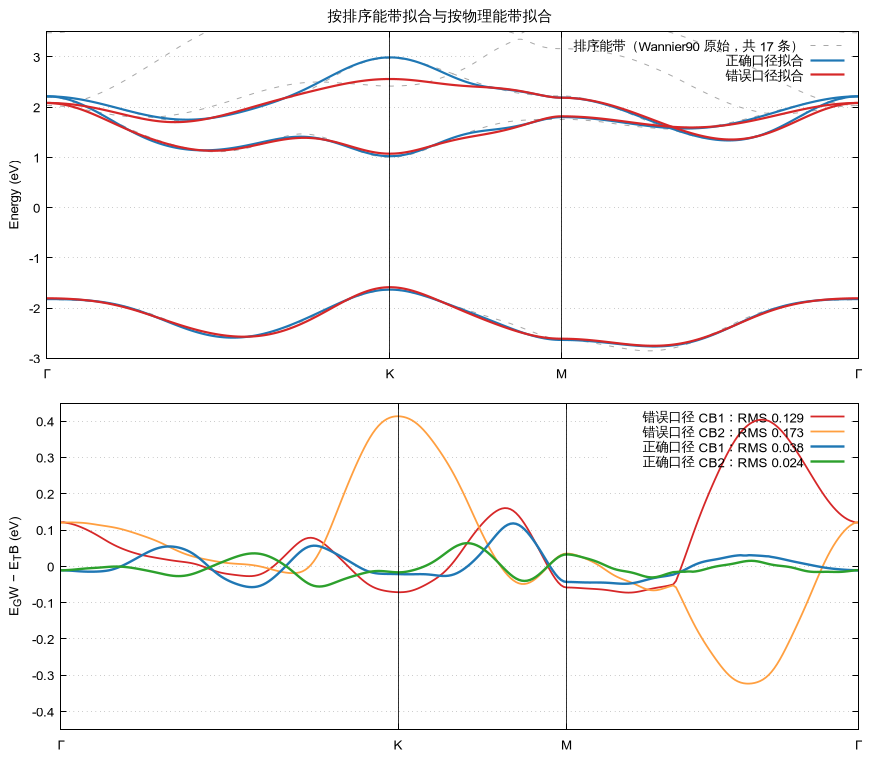
\includegraphics[width=0.84\textwidth]{fig_stitch.png}
\caption{两种口径的对比。每栏里实线是拟合目标，虚线是按该目标拟合出的结果，
浅色细虚线是同一窗口内没有参与拟合的其它能带。
(a) 目标取拼接后的物理能带；(b) 目标取按能量排序的能带。}
\label{fig:stitch}
\end{figure}

\subsection{导带配对}

拼接解决的是哪条是哪条，还剩下模型带对哪条物理带。
模型的两条导带在 $\Gamma$ 点严格简并，因为 $\eps_2$ 本身是二重简并的。
GW 数据里在 $\Gamma$ 点也简并的那两条物理带是拼接后的物理带 1 与物理带 3，
两者在 $\Gamma$ 点都是 2.2049~eV。
物理带 2 在 $\Gamma$ 点是 2.0331~eV，
来自 S 的 $p$ 轨道参与构成的另一条分支，不在三能带模型的基组内。
因此导带配对取物理带 1 与物理带 3，
模型带 2 对物理带 1，模型带 3 对物理带 3。

这个判断有独立的依据。
$K$ 谷附近模型的第二条导带能量较高。
以 $K$ 点为例，模型给出 2.990~eV，GW 的物理带 2 是 2.419~eV，相差 0.57~eV；
物理带 3 是 2.974~eV，只差 16~meV。
若强行配物理带 2，拟合残差会增大到 0.07~eV 以上。


%=====================================================================
\section{在 GW 能带上重新拟合参数\done}

\subsection{损失函数}

损失函数取均匀加权最小二乘，目标能带换成 GW 能带
\begin{equation}
f_{\mathrm{loss}}(\mathbf p)=\sum_{n\in\{\mathrm{VB},\mathrm{CB1},\mathrm{CB2}\}}\sum_{\kk}
\left[E_{\mathrm{TB}}(n,\kk;\mathbf p)-E_{\mathrm{GW}}(n,\kk)\right]^2 .
\label{eq:loss}
\end{equation}
两侧的能带都先经过第 4.3 节的拼接处理。
权重取均匀权重，不按能量加权，
理由是带边附近的绝对误差才是后面 BSE 关心的量。

参数向量 $\mathbf p$ 含 19 个分量，
分别是 $\eps_1$，$\eps_2$，六个 $t$，五个 $r$，六个 $u$。

\subsection{初值与优化}

初值取上一阶段用的那组文献参数\cite{liu2013}，先做一次最优刚性平移。
把 $\eps_1$ 与 $\eps_2$ 同时加上常数 $\Delta$ 等价于整条能带上移 $\Delta$，
因此 $\Delta$ 有闭式解
\begin{equation}
\Delta=\frac{1}{3N_k}\sum_{n,\kk}\left[E_{\mathrm{GW}}(n,\kk)-E_{\mathrm{TB}}(n,\kk)\right],
\end{equation}
不必交给优化器去爬。
这一步在本次计算里给出 $\Delta=-0.987$~eV，
它吸收的是两套能量零点之间的整体偏移。
带隙的张开不靠这一步，由后面的迭代调整 $\eps_1$ 与 $\eps_2$ 的差以及各跳跃项来完成。

优化采用逐参数扫描配合步长减半。
每一轮对 19 个参数依次尝试 $\pm\delta_j$，接受使损失函数下降的方向；
一轮结束后若没有改进，把所有步长减半，
直到最大步长小于 $10^{-6}$~eV。
这里不依赖梯度（不引入 Nelder-Mead、BFGS 这类优化库），
目的是把整个计算放进一个 C 程序里。
代价是收敛慢一些，第 1 轮之后损失函数下降得就不多了。

\subsection{结果}

拟合后的均方根偏差为 0.0334~eV，
分带为价带 0.0356~eV，第一导带 0.0385~eV，第二导带 0.0242~eV。
高对称点上的残差都在 $\pm0.04$~eV 以内（图~\ref{fig:fit}）。
残差主要来自模型本身，原因在第 3 节已经说明：
GW 修正不均匀，三能带模型吸收不了。

\begin{table}[htbp]
\centering
\caption{拟合到 GW 能带的三能带模型参数（单位 eV）。}
\label{tab:params}
\begin{tabular}{@{}ll@{}}
\toprule
原位能 & $\eps_1=-0.669051$,\quad $\eps_2=+0.909859$\\
\midrule
最近邻 & $t_{11}=-0.236031$,\ $t_{12}=+0.215955$,\ $t_{13}=-0.667015$,\\
       & $t_{22}=+0.081873$,\ $t_{23}=+0.201256$,\ $t_{33}=+0.092394$\\
次近邻 & $r_{11}=+0.124235$,\ $r_{12}=+0.292944$,\ $r_{21}=-0.136325$,\\
       & $r_{22}=-0.038118$,\ $r_{23}=+0.147411$\\
第三近邻 & $u_{11}=-0.079896$,\ $u_{12}=-0.123351$,\ $u_{13}=+0.034764$,\\
       & $u_{22}=+0.365806$,\ $u_{23}=-0.243409$,\ $u_{33}=-0.198801$\\
\bottomrule
\end{tabular}
\end{table}

这组参数是在绝对 GW 能量上得到的，$\eps_1$ 与 $\eps_2$ 含整体偏移，
不能与文献参数直接比较。
可比的是带隙。
拟合后的模型在 $K$ 点的带隙为 2.6548~eV，
GW 的直接带隙为 2.6416~eV，相差 13~meV。
这个差值会整体平移到后面所有的激子能级上。
\begin{figure}[H]
\centering
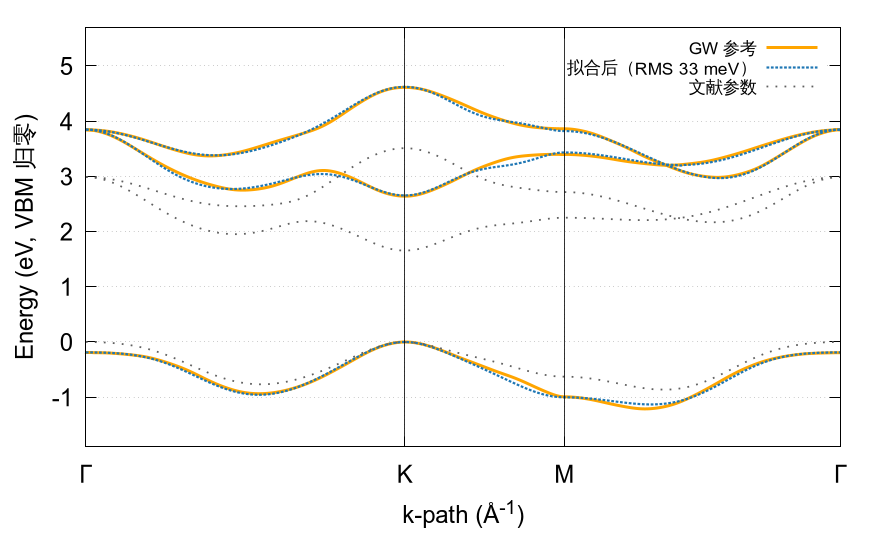
\includegraphics[width=0.82\textwidth]{fig_fit.png}
\caption{橙色是拟合目标（GW 参考能带），蓝色虚线是拟合结果，
灰色点线是初值，也就是上一阶段那个模型。
三组曲线都按各自的价带顶归零。}
\label{fig:fit}
\end{figure}


%=====================================================================
\section{介电屏蔽与 Keldysh 势\todo}
\label{sec:keldysh}

\subsection{二维体系的屏蔽}

三维体系的库仑势在动量空间是 $1/q^2$ 型。
单层材料的电场线可以穿出单层进入真空或衬底，屏蔽被削弱，
动量空间的相互作用在长波极限变成 $1/q$ 型，实空间则是对数型发散。
Keldysh 在研究薄金属膜时给出了这类势\cite{keldysh1979}，
Cudazzo 等人把它用到二维材料上\cite{cudazzo2011}。
动量空间的形式为
\begin{equation}
u(q)=-\frac{e^2}{2\eps_0\eps_d\,q\,\kappa(q)},
\qquad \kappa(q)=1+r_0q ,
\label{eq:keldysh}
\end{equation}
$r_0$ 是二维极化率对应的长度尺度，$\eps_d$ 是环境介电常数。
$q\to0$ 时 $\kappa\to1$，相互作用按 $1/q$ 发散。
这个发散是可积的，离散求和里却必须处理，见第~\ref{sec:reg}~节。

\subsection{\texorpdfstring{参数 $r_0$ 与介电环境}{参数 r0 与介电环境}}

设单层位于介电常数为 $\eps_1$ 的上方介质与 $\eps_3$ 的下方介质之间，
单层本身的等效厚度为 $d$、等效介电常数为 $\eps_2$。
有限厚度模型的解析结果为\cite{zhang2014}
\begin{equation}
r_0=\frac{2\eps_2^2-\eps_1^2-\eps_3^2}{2\eps_2(\eps_1+\eps_3)}\,d ,
\qquad
\eps_d=\frac{\eps_1+\eps_3}{2}.
\label{eq:r0}
\end{equation}
文献\cite{ridolfi2018}针对空气与二氧化硅的界面取
$\eps_1=1$，$\eps_3=4$，$\eps_2=12$，$d=6$~\AA{}，得到
\begin{equation}
\eps_d=2.5,\qquad r_0=13.55\ \text{\AA},\qquad \frac{2\pi r_0}{l}\approx 26.8 .
\end{equation}
这一组数对应 air/SiO$_2$ 环境。
作为对比基准的 VASP BSE 若用了别的介电环境，
$\eps_d$ 与 $r_0$ 需要按式~\eqref{eq:r0}~相应替换。

图~\ref{fig:keldysh}~给出了式~\eqref{eq:keldysh}~与裸库仑势的对比。
$q\ll1/r_0$ 时两者几乎重合，$q\gg1/r_0$ 时 Keldysh 势多出一个 $1/(r_0q)$ 因子，
下降得更快，屏蔽的效果正体现在这一段。

\begin{figure}[H]
\centering
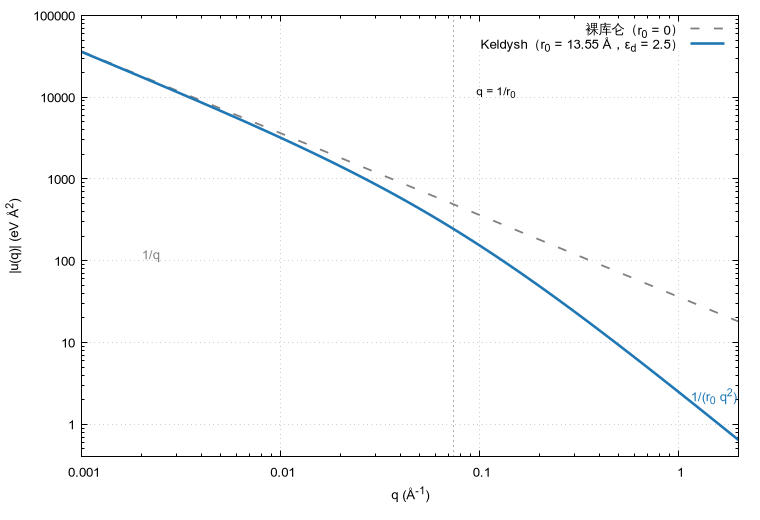
\includegraphics[width=0.64\textwidth]{fig_keldysh.png}
\caption{Keldysh 屏蔽势与裸库仑势的对比（双对数）。
取 $r_0=13.55$~\AA{}、$\eps_d=2.5$，竖线标出 $q=1/r_0$。}
\label{fig:keldysh}
\end{figure}

换到 eV 与 \AA{} 单位，取 $e^2/(4\pi\eps_0)=14.3996$~eV\AA{}，
式~\eqref{eq:keldysh}~写成
\begin{equation}
u(q)=-\frac{90.47}{\eps_d\,q\,(1+r_0q)}\ \text{eV}\,\text{\AA}^2
\qquad (q\ \text{以 \AA}^{-1}\ \text{为单位}).
\label{eq:keldysh_num}
\end{equation}

\subsection{实空间形式}

把式~\eqref{eq:keldysh}~作二维傅里叶变换，得到
\begin{equation}
u(r)=-\frac{e^2}{8\eps_0\eps_d r_0}
\left[H_0\!\left(\frac{r}{r_0}\right)-Y_0\!\left(\frac{r}{r_0}\right)\right],
\label{eq:keldysh_r}
\end{equation}
$H_0$ 与 $Y_0$ 分别是 Struve 函数与第二类 Bessel 函数。
$r\gg r_0$ 时 $u(r)\propto1/r$，$r\ll r_0$ 时按 $\log r$ 发散。
求解 BSE 时全程在动量空间使用式~\eqref{eq:keldysh}，
式~\eqref{eq:keldysh_r}~只用来核对量纲与长程行为。

%=====================================================================
\section{第二个目标：把式 (6) 的核算出来\todo}
\label{sec:bse}

这一节只做一件事：把论文式~(6) 的核矩阵元算出来。
写的时候按做题的顺序走：先说清楚已知什么、要求什么，再一步一步算，
每一步配一个能手算的小例子，最后把结果排成矩阵并检查。

\subsection{题目：已知、求、产出}

\textbf{已知。}
\begin{enumerate}
  \item 一个紧束缚哈密顿量 $H(\kk)$。把 $\kk$ 固定下来，它就是一个普通的有限维矩阵；
        本课题的模型是 $6\times6$（三个 $d$ 轨道乘两个自旋）。
  \item 每个 $\kk$ 点上解出来的本征值 $\eps_{n\kk}$ 与本征矢 $C^{n}_{\alpha\kk}$。
        这里 $n$ 是能带编号，$\alpha$ 是轨道编号。
  \item 屏蔽库仑势 $u(q)$ 的表达式，以及 $r_0$、$\eps_d$ 两个介电参数（第~\ref{sec:keldysh}~节）。
\end{enumerate}

\textbf{求。}
对所有 $\kk$、$\kq$，以及所有导带 $c,c'$ 与价带 $v,v'$，算出
\begin{equation}
W^{(d)}_{cv\kk,c'v'\kq}=u(\kk-\kq)\,I^{*}_{c'\kq,c\kk}\,I_{v'\kq,v\kk},
\label{eq:kernel}
\end{equation}
这就是论文的式~(6)。$I$ 叫轨道交叠，下一步会给定义。

\textbf{产出。}
一个方阵，行和列都用三元组 $(\kk,c,v)$ 编号，维数
\begin{equation*}
N_{\mathrm{tot}}=N_k^2\times N_c\times N_v .
\end{equation*}
这个方阵加上对角项 $E_{cv\kk}=\eps_{c\kk}-\eps_{v\kk}$，
就是目标二要交给目标三的东西。

这个核用在哪里，先交代一句，省得算完不知道干什么用。
激子态写成电子-空穴对的线性组合
\begin{equation}
|M\rangle=\sum_{cv\kk}A^{M}_{cv\kk}\,|v\kk\to c\kk\rangle ,
\label{eq:basis}
\end{equation}
代入多体薛定谔方程后得到本征方程
\begin{equation}
E_{cv\kk}A^{M}_{cv\kk}
+\frac{1}{V}\sum_{c'v'\kq}W_{cv\kk,c'v'\kq}A^{M}_{c'v'\kq}
=E_{M}A^{M}_{cv\kk},
\qquad V=A_cN_k^2 ,
\label{eq:bse}
\end{equation}
也就是论文的式~(5)。式~\eqref{eq:kernel}~是它左边的核；
怎么解式~\eqref{eq:bse}~属于目标三，这里不展开。

\subsection{符号对照表}

\begin{table}[htbp]
\centering
\caption{式~\eqref{eq:kernel}~里出现的符号。最后一列是本课题模型的实际取值。}
\label{tab:symbols}
\begin{tabular}{@{}lll@{}}
\toprule
符号 & 含义 & 本课题取值\\
\midrule
$\kk,\kq$ & 布里渊区里的两个 $k$ 点 & 均匀网格，共 $N_k^2$ 个\\
$c,c'$ & 导带编号 & 2 条\\
$v,v'$ & 价带编号 & 1 条\\
$\alpha$ & 轨道编号 & 6 个（3 个 $d$ 轨道 $\times$ 2 个自旋）\\
$C^{n}_{\alpha\kk}$ & 第 $n$ 条带在轨道 $\alpha$ 上的分量 & 复数，$|C|\le1$\\
$\eps_{n\kk}$ & 第 $n$ 条带的能量 & eV\\
$u(q)$ & 屏蔽库仑势 & eV$\cdot$\AA$^2$\\
$I$ & 两条 Bloch 态的轨道交叠 & 无量纲，$|I|\le1$\\
$N_k$ & 每个方向的 $k$ 点数 & 文献取 60\\
$A_c$ & 原胞面积 $\sqrt3a^2/2$ & $8.65$~\AA$^2$\\
$V$ & 晶体总面积 $A_cN_k^2$ & $N_k=60$ 时 $3.1\times10^4$~\AA$^2$\\
\bottomrule
\end{tabular}
\end{table}

\subsection{第一步：解 $H(\kk)$，得到本征值和本征矢}

对每个 $\kk$ 点解本征值问题
\begin{equation}
H(\kk)\,\mathbf u_{n\kk}=\eps_{n\kk}\,\mathbf u_{n\kk},
\qquad
\mathbf u_{n\kk}=\big(C^{n}_{1\kk},C^{n}_{2\kk},\dots,C^{n}_{\alpha\kk},\dots\big)^{T}.
\label{eq:eig}
\end{equation}
$\mathbf u_{n\kk}$ 是一个列向量，长度等于轨道数（本课题是 6）。
解一次得到一个本征值和对应的一个本征矢；把 $6$ 个都解出来，
就得到 $6$ 个 $\eps_{n\kk}$ 和 $6$ 个长度为 6 的列向量。

小例子：先看一个能手算的 $2\times2$ 情形，
\begin{equation*}
H=\begin{pmatrix}2&1\\[1pt]1&3\end{pmatrix}.
\end{equation*}
解本征值的方程是 $\det(H-\lambda I)=0$，即
\begin{equation*}
(2-\lambda)(3-\lambda)-1=\lambda^2-5\lambda+5=0
\;\Longrightarrow\;
\lambda=\frac{5\pm\sqrt5}{2}=3.618,\ 1.382 .
\end{equation*}
把 $\lambda=1.382$ 代回 $(H-\lambda I)\mathbf u=0$，第一行给出
$0.618\,u_1+u_2=0$，取 $u_1=1$ 得 $u_2=-0.618$。
归一化（让 $u_1^2+u_2^2=1$）得到
\begin{equation*}
\mathbf u_1=(0.851,\,-0.526)^T,\qquad
\mathbf u_2=(0.526,\,0.851)^T .
\end{equation*}
这两个向量正交：$0.851\times0.526+(-0.526)\times0.851=0$。

本课题的 $6\times6$ 矩阵不方便手算，交给数值对角化。
要点只有一条：解出来的本征矢必须归一化，否则后面算出的交叠积分会整体偏大或偏小。

\subsection{第二步：把本征矢的相位定死}

本征矢不是唯一的。$\mathbf u$ 是本征矢，$e^{\ii\varphi}\mathbf u$ 也是：
\begin{equation*}
H\,(e^{\ii\varphi}\mathbf u)=e^{\ii\varphi}H\mathbf u
=e^{\ii\varphi}\eps\,\mathbf u=\eps\,(e^{\ii\varphi}\mathbf u).
\end{equation*}
$\varphi$ 可以随便取，这个自由度叫相位任意性。
数值对角化每次给的 $\varphi$ 都不一样，必须先把它定下来，
否则后面算出的交叠积分每次都不同。

定法是这样：把每条带在轨道上的分量加起来，得到一个复数
\begin{equation}
S_{n\kk}=\sum_{\alpha}C^{n}_{\alpha\kk},
\label{eq:S}
\end{equation}
要求这个和的辐角为零。做法是把整条带乘上 $e^{-\ii\arg S_{n\kk}}$：
\begin{equation}
C^{n}_{\alpha\kk}\;\longrightarrow\;C^{n}_{\alpha\kk}\,e^{-\ii\arg S_{n\kk}},
\qquad\text{从而}\qquad
\sum_{\alpha}C^{n}_{\alpha\kk}\in\mathbb{R}.
\label{eq:gauge}
\end{equation}

小例子：取
$\mathbf C=\frac{1}{\sqrt2}(1,\ \ii)^T$，它是归一化的（$\frac12+\frac12=1$）。
求和得
$S=\frac{1}{\sqrt2}(1+\ii)$，模长是 1，辐角是 $\pi/4$。
乘上 $e^{-\ii\pi/4}$ 之后
\begin{equation*}
\mathbf C=\frac{1}{\sqrt2}e^{-\ii\pi/4}(1,\ \ii)^T
=(0.5-0.5\ii,\ 0.5+0.5\ii)^T ,
\end{equation*}
两个分量之和等于 $1$，是实数，相位定住了；归一化没有变（$0.5+0.5=1$）。

要注意的是，如果某条带在所有轨道上的分量加起来恰好为零，
$S_{n\kk}=0$，辐角无法定义，这个办法失效。
这时改用"平行移动"：让这条带在相邻 $k$ 点上的内积为正实数，逐点定相位。

\subsection{第三步：算轨道交叠积分 $I$}

定义是两个 Bloch 态在轨道上的重叠
\begin{equation}
I_{a\kq,b\kk}=\sum_{\alpha}C^{a*}_{\alpha\kq}\,C^{b}_{\alpha\kk}.
\label{eq:overlap}
\end{equation}
把它看成两个长度为 6 的复向量的内积：$\kq$ 点第 $a$ 条带的向量与 $\kk$ 点第 $b$ 条带的向量，
逐分量相乘（第一个取复共轭）再相加。
$I=1$ 表示两个态完全一样，$I=0$ 表示正交，一般介于两者之间。

小例子：取
$\mathbf a=\frac{1}{\sqrt2}(1,\ \ii)^T$，
$\mathbf b=\frac{1}{\sqrt2}(1,\ 1)^T$，则
\begin{equation*}
I=\bar a_1b_1+\bar a_2b_2
=\frac{1}{\sqrt2}\cdot\frac{1}{\sqrt2}
+\frac{-\ii}{\sqrt2}\cdot\frac{1}{\sqrt2}
=0.5-0.5\ii ,
\qquad |I|^2=0.5 .
\end{equation*}

三条可以直接拿来检查程序的性质：
\begin{enumerate}
  \item 同一个 $k$ 点上同一条带：$I_{a\kk,a\kk}=\sum_\alpha|C^{a}_{\alpha\kk}|^2=1$（归一化）。
  \item 同一个 $k$ 点上不同能带：$I_{a\kk,b\kk}=0$（本征矢互相正交）。
  \item 交换上下指标取复共轭：
        \begin{equation}
        I_{a\kq,b\kk}=I^{*}_{b\kk,a\kq} .
        \label{eq:I_herm}
        \end{equation}
\end{enumerate}
第一条最容易查：程序跑完，$I_{a\kk,a\kk}$ 与 1 的差有多大，就直接反映对角化的精度。

\subsection{第四步：算屏蔽库仑势 $u(q)$}

二维体系的屏蔽势取 Keldysh 形式（第~\ref{sec:keldysh}~节，论文式~(8)--(10)）
\begin{equation}
u(q)=-\frac{e^2}{2\eps_0\eps_d\,q\,\big(1+r_0q\big)},
\qquad
\eps_d=\frac{\eps_1+\eps_3}{2},
\qquad
r_0=\frac{2\eps_2^2-\eps_1^2-\eps_3^2}{2\eps_2(\eps_1+\eps_3)}\,d .
\label{eq:keldysh2}
\end{equation}
这里的 $q$ 不是一维的数，而是两个 $k$ 点之差的长度
\begin{equation}
q=|\kk-\kq|=\sqrt{(k_x-k'_x)^2+(k_y-k'_y)^2}.
\label{eq:qmod}
\end{equation}
$u$ 只依赖这个长度，与方向无关，所以可以预先按 $q$ 做成表，需要时查表。

数值代入：空气/二氧化硅界面取 $\eps_1=1$、$\eps_3=4$，于是 $\eps_d=2.5$；
单层厚度 $d=6$~\AA{}、介电常数 $\eps_2=12$，代入上式得 $r_0=13.55$~\AA{}。
用 $e^2/(4\pi\eps_0)=14.4$~eV$\cdot$\AA{}，则
\begin{equation*}
\frac{e^2}{2\eps_0\eps_d}=2\pi\times\frac{14.4}{2.5}=36.2\ \text{eV}\cdot\text{\AA},
\end{equation*}
于是
\begin{equation*}
u(q)=-\frac{36.2}{q\,(1+13.55\,q)}\ \text{eV}\cdot\text{\AA}^2
\qquad (q\ \text{以 \AA}^{-1}\ \text{为单位}).
\end{equation*}
代入几个值感受一下量级：$q=0.2$~\AA$^{-1}$ 时 $u=-48.8$~eV$\cdot$\AA$^2$；
$q=1/r_0=0.0738$~\AA$^{-1}$ 时 $u=-245$~eV$\cdot$\AA$^2$；
$q$ 越小 $u$ 越大，$q\to0$ 时发散——这正是第六步要处理的麻烦。

两个区域：$r_0q\ll1$ 时分母约为 $q$，$u\propto1/q$，对应实空间的长程 $1/r$；
$r_0q\gg1$ 时分母约为 $r_0q^2$，$u\propto1/q^2$。
两者的分界在 $q\approx1/r_0=0.074$~\AA$^{-1}$。

\subsection{第五步：把三个数乘起来}

到这一步三样东西都有了：$u(\kk-\kq)$ 是一个实数，
$I_{c'\kq,c\kk}$ 与 $I_{v'\kq,v\kk}$ 是两个复数。按式~\eqref{eq:kernel}~相乘即可：
\begin{equation*}
W^{(d)}_{cv\kk,c'v'\kq}
=\underbrace{u(\kk-\kq)}_{\text{实数}}\cdot
\underbrace{I^{*}_{c'\kq,c\kk}}_{\text{复数}}\cdot
\underbrace{I_{v'\kq,v\kk}}_{\text{复数}} .
\end{equation*}
乘积一般仍是复数，因为两个 $I$ 来自不同的带。

小例子：设某个 $(\kk,\kq)$ 对上 $u=-245$~eV$\cdot$\AA$^2$，
$I_{c'\kq,c\kk}=0.5-0.5\ii$，$I_{v'\kq,v\kk}=1$（同一个价带、$\kq$ 与 $\kk$ 很接近时的极限），则
\begin{equation*}
W^{(d)}=(-245)\times(0.5+0.5\ii)\times1
=-122.5\,(1+\ii)\ \text{eV}\cdot\text{\AA}^2 .
\end{equation*}
别忘了式~\eqref{eq:bse}~里还有一个 $1/V$。$N_k=60$ 时 $V=A_cN_k^2=8.65\times3600=3.1\times10^4$~\AA$^2$，
所以矩阵里实际存的是
\begin{equation*}
\frac{W^{(d)}}{V}=\frac{-122.5(1+\ii)}{3.1\times10^4}
\approx-3.9\times10^{-3}(1+\ii)\ \text{eV},
\end{equation*}
也就是几 meV 的量级。单个矩阵元是 meV 量级，
但求和有 $N_k^2N_cN_v$ 项，最后能给出几百 meV 的束缚能，量级上是自洽的。

\subsection{第六步：$\kk=\kq$ 的对角元要单独处理}
\label{sec:reg}

式~\eqref{eq:qmod}~在 $\kq=\kk$ 时给出 $q=0$，
而式~\eqref{eq:keldysh2}~在 $q=0$ 处分母为零，$u$ 发散。
矩阵的对角块里全是这种项，不能直接丢，也不能直接算。

处理办法是把它换成 $q=0$ 附近一个小区域上的平均值（论文式~(17)）
\begin{equation}
u(\qq\approx0)\;\longrightarrow\;\frac{1}{\Delta q}\int_{\Delta q}u(\qq)\,\dd\qq
\approx\frac{c\,aN_k}{2\pi}\left[\alpha_1+\alpha_2\frac{2\pi r_0}{aN_k}
+\alpha_3\left(\frac{2\pi r_0}{aN_k}\right)^2\right],
\qquad c\equiv-\frac{e^2}{2\eps_0\eps_d} .
\label{eq:reg}
\end{equation}
$\Delta q$ 是每个 $k$ 点在倒空间里代表的面积；$\alpha_{1,2,3}$ 是常数，
由这个小区域的形状和展开到几阶决定。

展开参数是
\begin{equation*}
\frac{2\pi r_0}{aN_k}=\frac{26.9}{N_k},\qquad N_k=60\ \text{时等于}\ 0.45 .
\end{equation*}
$0.45$ 不算小，所以 $\alpha_2$、$\alpha_3$ 两项不能随便丢。
这解释了论文图~2 的现象：只留 $\alpha_1$（相当于 $\alpha_{2,3}=0$）时收敛明显慢，
因为被丢掉的项在 $N_k=60$ 附近还有百分之几十的贡献。

本课题的做法是直接对式~\eqref{eq:reg}~里的积分做数值求积，
不引入拟合系数，从而把"用哪一组 $\alpha$"这个问题绕开。

\subsection{第七步：把矩阵元排成矩阵}

现在有了一堆数 $W^{(d)}_{cv\kk,c'v'\kq}$，要把它们放到矩阵的确定位置上。
先给每个三元组 $(\kk,c,v)$ 编一个行号。设 $k$ 点在网格上的线性编号是 $i_k$（从 0 开始），
规则是
\begin{equation}
\text{行号}=i_k\,(N_cN_v)+i_c\,N_v+i_v .
\label{eq:index}
\end{equation}
列号用同样的规则给 $(\kq,c',v')$ 编。

小例子：取 $N_k=2$（网格 $2\times2$，共 4 个 $k$ 点）、$N_c=2$、$N_v=1$，
矩阵维数 $N_{\mathrm{tot}}=4\times2\times1=8$。
三元组 $(\kk_2,c=1,v=0)$ 的行号是 $2\times2+1\times1+0=5$。

排好之后，式~\eqref{eq:bse}~可以写成标准的矩阵本征值问题
\begin{equation}
\mathcal{H}\mathbf A=E\mathbf A,
\qquad
\mathcal{H}_{(c\kk),(c'\kq)}
=\delta_{cc'}\delta_{\kk\kq}E_{cv\kk}
+\frac{1}{A_cN_k^2}\,u(\kk-\kq)\,I^{*}_{c'\kq,c\kk}\,I_{v'\kq,v\kk}.
\label{eq:bse_matrix}
\end{equation}

$W$ 是厄米矩阵，这一点可以直接验：把行列交换并对整体取复共轭，
由式~\eqref{eq:I_herm}~的 $I_{a\kq,b\kk}=I^{*}_{b\kk,a\kq}$ 与 $u(-\qq)=u(\qq)$ 得到
\begin{equation*}
\left[\mathcal{H}_{(c'\kq),(c\kk)}\right]^{*}
=\left[\delta_{cc'}\delta_{\kk\kq}E_{c'\kq}\right]^{*}
+\frac{1}{A_cN_k^2}u(\kq-\kk)\,I_{c\kk,c'\kq}\,I_{v\kk,v'\kq}
=\mathcal{H}_{(c\kk),(c'\kq)} .
\end{equation*}
厄米这一点很重要：它保证解出来的 $E_M$ 是实数。

\subsection{检查答案}

题目做完要验算。这一步有四条检查，按顺序做。

\begin{enumerate}
  \item \textbf{归一化检查。} 对每条带、每个 $k$ 点算 $I_{a\kk,a\kk}$，它应当等于 1。
        偏离 1 的量级就是对角化的精度。
  \item \textbf{相位检查。} 固定相位前后，$I_{n\kk',n\kk}$ 的相位不应跳变；
        相邻 $k$ 点上它的模应当接近 1 并逐渐下降。
        若相位随机跳，说明第二步没做对。
  \item \textbf{厄米检查。} 抽若干对矩阵元，验 $\mathcal{H}_{ij}=\mathcal{H}^{*}_{ji}$。
        不成立通常是行号编错，或 $I$ 的复共轭取反了。
  \item \textbf{收敛检查。} 把 $N_k$ 从 30 加到 60，看最低激子能级
        是否单调地趋于稳定值。正则化方案选择不当会让它收敛很慢或来回摆。
        判断实现对不对，看的是这条曲线，而不是单个 $N_k$ 下的数字。
\end{enumerate}

四条都过了，才算把式~\eqref{eq:kernel}~算对，可以交给目标三去解式~\eqref{eq:bse}。

\section{光学响应\todo}

有了本征值与本征矢，线性电导率由费米黄金规则给出
\begin{equation}
\operatorname{Re}\sigma(\omega)=\frac{e^2\pi}{m^2\hbar\omega V}
\sum_M\left|\langle\mathrm{FS}|\hat P_x|M\rangle\right|^2
\delta(\omega-\omega_M),
\label{eq:sigma}
\end{equation}
$\mathrm{FS}$ 是基态，$\hat P_x$ 是总动量算符的 $x$ 分量。
把式~\eqref{eq:basis}~代入，并利用单粒子矩阵元与速度算符的关系
\begin{equation}
\langle\mathrm{FS}|\hat P_x a^\dagger_{c\kk}a_{v\kk}|\mathrm{FS}\rangle
=\langle\psi_{v\kk}|\hat p_x|\psi_{c\kk}\rangle
=\frac{m}{\hbar}\langle\psi_{v\kk}|\nabla_{k_x}\hat H(\kk)|\psi_{c\kk}\rangle ,
\label{eq:velocity}
\end{equation}
电导率写成
\begin{equation}
\operatorname{Re}\sigma(\omega)=\frac{e^2}{4\hbar}\frac{4\pi}{\hbar\omega V}
\sum_M\left|
\sum_{cv\kk}A^{M}_{cv\kk}
\sum_{\alpha\beta}C^{v*}_{\alpha\kk}C^{c}_{\beta\kk}
\langle\phi_\alpha|\nabla_{k_x}\hat H(\kk)|\phi_\beta\rangle
\right|^2\delta(\hbar\omega-\hbar\omega_M).
\label{eq:sigma_explicit}
\end{equation}
速度矩阵元由哈密顿量对 $k$ 的解析导数给出，不需要数值差分。
式~\eqref{eq:sigma_explicit}~同时给出每个激子态的振子强度，
这是判断亮态与暗态的依据。

本篇的对比目标是激子能级，第~\ref{sec:bse}~节的本征值已经够用。
式~\eqref{eq:sigma_explicit}~留作下一步，用于把计算谱与实验吸收谱对照。

%=====================================================================
\section{理论公式与程序的对应}

表~\ref{tab:map}~列出各部分公式在程序中的位置。
单粒子部分已经实现，BSE 部分正在实现。

\begin{table}[htbp]
\centering
\caption{公式与程序模块的对应关系。}
\label{tab:map}
\begin{tabular}{lll}
\toprule
内容 & 公式 & 程序位置\\
\midrule
Bloch 哈密顿量 & 式~\eqref{eq:hk} & \texttt{src/tb.c: tb\_build\_Hk}\\
跳跃矩阵与对称性 & 式~\eqref{eq:sym},~\eqref{eq:hop} & \texttt{src/tb.c: generate\_hopping\_matrices\_*}\\
自旋轨道耦合 & 式~\eqref{eq:soc} & \texttt{src/tb.c: tb\_eig\_soc}\\
本征值与本征矢 & & \texttt{src/herm3.c: herm3\_jacobi}\\
能带拼接 & 第 4.3 节 & \texttt{src/bandtrack.c: band\_track}\\
参数拟合 & 式~\eqref{eq:loss} & \texttt{opt\_main.c}\\
屏蔽势 & 式~\eqref{eq:keldysh_num} & 待实现\\
交叠积分与规范固定 & 式~\eqref{eq:overlap},~\eqref{eq:gauge} & 待实现\\
BSE 矩阵 & 式~\eqref{eq:bse_matrix} & 待实现\\
库仑奇点正则化 & 式~\eqref{eq:reg} & 待实现\\
光学响应 & 式~\eqref{eq:sigma_explicit} & 待实现\\
\bottomrule
\end{tabular}
\end{table}

%=====================================================================
\section{收敛性与误差来源}

判断实现是否正确，除了核对公式，还要看几个可以独立验证的极限。

\paragraph{无相互作用极限}
把 $u$ 置零后，式~\eqref{eq:bse_matrix}~退化为对角矩阵，
本征值应当精确等于单粒子跃迁能 $\eps_{c\kk}-\eps_{v\kk}$ 的集合。
这是验证矩阵装配与索引映射最直接的方法。

\paragraph{谷简并}
无 SOC 时 $K$ 与 $K'$ 完全对称，最低激子应当是二重简并的。
VASP 的 BSE 结果同样给出成对的简并本征值，前两条相差不到 $10^{-8}$~eV，
可以拿来对照。

\paragraph{网格收敛}
最低激子能量随 $N_k$ 的变化应当单调趋于稳定值。
正则化方案决定收敛速度，$2\pi r_0/l\approx26.8$ 意味着 $N_k$ 只有几十时，
$q\to0$ 附近的处理仍在显著影响结果。
判断收敛的依据是相邻 $N_k$ 之间的差值，而非绝对精度。

\paragraph{误差来源}
拟合给出的带隙比 GW 小 13~meV，这一项整体平移到所有激子能级上。
三能带模型缺少 S、$p$ 导出的那条分支，对高能激子的影响比对最低激子大。
忽略 $Q\ne0$ 的矩阵元会系统性影响束缚能，
文献\cite{ridolfi2018}把采样域取成第一布里渊区，以保证这部分可以忽略。
简并点附近的规范不唯一会带来不可控的小扰动，
可以通过改变锚点或相位约定估计其量级。

%=====================================================================
\section{小结}

这一篇把上一篇的三能带模型推到了激子层面。
单粒子部分换成 GW 准粒子能带重新拟合，
19 个参数在 285 个 $k$ 点上的均方根偏差为 33~meV，
$K$ 点带隙 2.6548~eV 与 GW 的 2.6416~eV 相差 13~meV。
相互作用部分引入 Keldysh 型二维屏蔽势，
环境取 air/SiO$_2$，给出 $\eps_d=2.5$、$r_0=13.55$~\AA{}。
激子用 TDA 下的 BSE 求解，核保留直接项与轨道交叠，
规范按分量之和为实数固定，$q\to0$ 的奇点用小区间平均正则化。

剩下的工作是数值实现与对照。
判断结果是否可信，先看无相互作用极限与谷简并这两个必要条件，
再看最低激子随 $N_k$ 的收敛。

%=====================================================================
\begin{thebibliography}{99}

\bibitem{ridolfi2018}
M.~Ridolfi, C.~Lewenkopf, and V.~M.~Pereira,
Excitonic structure of the optical conductivity in MoS$_2$ monolayers,
Phys. Rev. B \textbf{97}, 205409 (2018).

\bibitem{liu2013}
G.-B.~Liu, W.-Y.~Shan, Y.~Yao, W.~Yao, and D.~Xiao,
Three-band tight-binding model for monolayers of group-VIB transition metal dichalcogenides,
Phys. Rev. B \textbf{88}, 085433 (2013).

\bibitem{rohlfing2000}
M.~Rohlfing and S.~G.~Louie,
Electron-hole excitations and optical spectra from first principles,
Phys. Rev. B \textbf{62}, 4927 (2000).

\bibitem{keldysh1979}
L.~V.~Keldysh,
Coulomb interaction in thin semiconductor and semimetal films,
JETP Lett. \textbf{29}, 658 (1979).

\bibitem{cudazzo2011}
P.~Cudazzo, I.~V.~Tokatly, and A.~Rubio,
Dielectric screening in two-dimensional insulators,
Phys. Rev. B \textbf{84}, 085406 (2011).

\bibitem{zhang2014}
C.~Zhang, A.~Johnson, C.-L.~Hsu, L.-J.~Li, and C.-K.~Shih,
Direct imaging of four-particle states in monolayer MoS$_2$,
Nano Lett. \textbf{14}, 2443 (2014).

\bibitem{berkelbach2013}
T.~C.~Berkelbach, M.~S.~Hybertsen, and D.~R.~Reichman,
Theory of neutral and charged excitons in monolayer transition metal dichalcogenides,
Phys. Rev. B \textbf{88}, 045318 (2013).

\bibitem{wu2015}
F.~Wu, F.~Qu, and A.~H.~MacDonald,
Exciton band structure of monolayer MoS$_2$,
Phys. Rev. B \textbf{91}, 075310 (2015).

\bibitem{li2014}
Y.~Li, A.~Chernikov, X.~Zhang, A.~Rigosi, H.~M.~Hill, A.~M.~van der Zande,
D.~A.~Chenet, E.-M.~Shih, J.~Hone, and T.~F.~Heinz,
Measurement of the optical dielectric function of monolayer transition-metal dichalcogenides,
Phys. Rev. B \textbf{90}, 205422 (2014).

\bibitem{qiu2013}
D.~Y.~Qiu, F.~H.~da Jornada, and S.~G.~Louie,
Optical spectrum of MoS$_2$: Many-body effects and diversity of exciton states,
Phys. Rev. Lett. \textbf{111}, 216805 (2013).

\end{thebibliography}

\end{document}
